\subsection{Разработка технического задания}
\subsubsection{Постановка задачи проектирования}

Целью разработки подсистемы автономного определения перемещения объекта является предоставления удобного с точки зрения интеграции компонента для встраивания во многие бытовые автономные автоматические системы,  в то же время дешевого и не требующего специализированных устройств для своей работы.

\subsubsection{Описание предметной области}
\paragraph{Естественно-языковое описание процесса.}

В ходе создания подвижных автономных систем возникает задача определения текущего местоположения объекта в пространстве.

Для этого можно использовать различные методы, основанные на глобальном позиционировании в географической системе координат с использованием позиционирования по спутникам (GPS, ГЛОНАСС), или методы, основанные на определении перемещения от стартовой позиции. При этом у данных методов разные сферы применения. Так, например, при позиционировании внутри помещения использование спутниковых систем позиционирвоания становиться невозможным по причине слабого сигнала или его полного отсутсвтвия, а так же из-за недостаточной точности в рамках навигации внутри интерьера помещения. Так же не стоит забывать про акутальность систем навигации в космической отрасли, где использование спутников является невозможным впринципе. 
Вторую группу методов принято называть методами одометрии, которые могут быть основаны на:
\begin{itemize}
\item на вращении колес;
\item использовании инерциальных измерительных приборов;
\item компьютерном зрении.
\end{itemize}

Каждый из них обладает своими плюсами и минусами \cite{odometryMethods}, но развитие вычислительной техники и алгоритмов компьютерного зрения дало мощный толчок к более широкому применению визуальной одометрии. Данный подход позволяет получать один видеоряд через видеокамеру и на его основе получать разные сведения об окружающей среде. Тем не менее он не лишен недостатков. Для борьбы с ними применяется комбинация нескольких методов одомтерии. 

Одним из вариантов сомещения методов является использование метода визуальной одометрии и инерционных измерительных устройств. 

При таком гибридном методе данные с видеокамеры и данные с инерционных измерительных устройств обрабатываются параллельно и независимо. В результате получаются два независимых рассчитынных положения носителя, после чего они сопоставляются, и из них выбираются наиболее правдоподобные. 

Таким образом, в процессе функционирования спроектированного модуля визуальной одометрии происходит следующий бесконечный процесс. 
На вход модуля непрерывно подается видео поток и данные об угловых скоростях и ускорении объекта относительно трех взаимноперпендикулярных осей. Эти данные обрабатываются параллельно в соответствующих модулях, на выходе каждого из которых получаем смещение объекта относительно предыдущего положения и его поворот. Далее эти данные совмещаются и выбираются наиболее правдоподобные, которые затем прибавляются к положению и углу поворота, высчитанным на предыдущей итерации. 


\paragraph{Графическое представление процесса}
Графическое представление процесса процесса представлено на рисунке~\ref{pic:predmetOblast}.

\begin{figure}[!htb]
\center{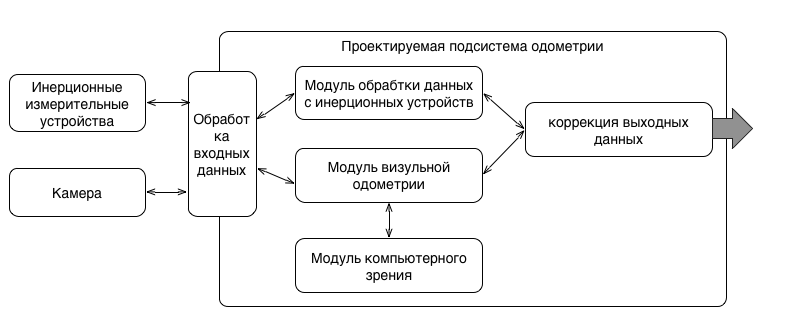
\includegraphics[width=0.8\linewidth]{pics/predmetOblast.png}}
\caption{Графическое представление процесса.}
\label{pic:predmetOblast}
\end{figure}

\paragraph{Вычисление оптического потока.}

\textbf{Оптический поток} — это изображение видимого движения объектов, поверхностей или краев сцены, получаемое в результате перемещения наблюдателя (глаз или камеры) относительно сцены\cite{wikiOpticalFlow}.

Существует несколько подходов к определению смещений между двумя соседними кадрами. Например, можно для каждого небольшого фрагмента (скажем, 8 на 8 пикселей) одного кадра найти наиболее похожий фрагмент на следующем кадре. В этом случае разность координат исходного и найденного фрагментов даст нам смещение. Основная сложность тут состоит в том, как быстро отыскать нужный фрагмент, не перебирая весь кадр пиксель за пикселем. Различные реализации этого подхода так или иначе решают проблему вычислительной сложности. Некоторые настолько успешно, что применяются, например, в распространенных стандартах сжатия видео. Платой за скорость естественно является качество. Мы же рассмотрим другой подход, который позволяет получить смещения не для фрагментов, а для каждого отдельного пикселя, и применяется тогда, когда скорость не столь критична. Именно с ним в литературе часто связывают термин “оптический поток”.

Данный подход часто называют дифференциальным, поскольку в его основе лежит вычисление частных производных по горизонтальному и вертикальному направлениям изображения. Как мы увидим далее, одних только производных недостаточно чтобы определить смещения. Именно поэтому на базе одной простой идеи появилось великое множество методов, каждый из которых использует какую-нибудь свою математическую пляску с бубном, чтобы достичь цели. Сконцентрируемся на методе Лукаса-Канаде (Lucas-Kanade), предложенном в 81 году Брюсом Лукасом и Такео Канаде. Данный метод является наименее ресурсоемким  \cite{habrOpticalFlowAbout} при этом обеспечивает приемлемое качество вычисления оптического потока. 

С математической точки зрения данный алгоритм можно описать следующим образом.
Пусть даны два изображения $F1$ и $F2$, и нам требуется найти смещение точки с координотой $x$. Рассматривая два последовательных изображения можно сказать:
$$ f_2(x) = f_1 (x-d)$$
Обратите внимание, что $f_1$ и $f_2$ при желании можно записать и в общем виде: $f_1(x) = I (x, y, t)$ ; $f_2(x) = I (x, y, t+1)$.

Свяжем известные значения со смещением d. Для этого запишем разложение в ряд Тейлора для $ f_1 (x-d)$:
$$  f_1 (x-d) =f_1(x) + df_1'(x) + O(d^2f_1'') $$
Предположим, что $ f_1 (x-d)$ достаточно хорошо аппроксимируется первой производной. Сделав это предположение, отбросим всё что после первой производной:
$$  f_1 (x-d) =f_1(x) + df_1'(x) $$

Смещение $d$ — это наша искомая величина, поэтому необходимо преобразовать $ f_1 (x-d)$ . Как мы условились ранее, $ f_2(x) = f_1 (x-d) $, поэтому просто перепишем:
$$ f_2(x)= f_1(x) - df_1'(x) $$
Отсюда следует:
$$ d = \frac{f_1(x)-f_2(x)}{f_1'(x)} $$

Следует отметить, что выше был рассмотрен одномерный случай и были сделаны несколько грубых допущений. Но описание алгоритма Лукаса-Канаде для двумерного случая только усложняет математические выводы и понимание сути. 

Для снижения погрешности вызванной отбрасыванием старших производных смещение для каждой пары кадров (назовём их $F_i$ и $F_{i+1}$) можно вычислять итеративно. В литературе это называется искажением (warping). На практике это означает, что, вычислив смещения на первой итерации, мы перемещаем каждый пиксель кадра $F_{i+1}$ в противоположную сторону так, чтобы это смещение компенсировать. На следующей итерации вместо исходного кадра $F_{i+1}$ мы будем использовать его искаженный вариант $F_{i+1}^1$. И так далее, пока на очередной итерации все полученные смещения не окажутся меньше заданного порогового значения. Итоговое смещение для каждого конкретного пикселя мы получаем как сумму его смещений на всех итерациях \cite{habrOpticalFlowTheory}.

Так же следует отметить, что данный алгоритм плохо работает на однотонных изображениях. Данный недостаток является самым критичным. 

\paragraph{Одометрия с использованием инерциальных измерительных устройств}
Навигационные решения надлежащего качества могут быть получены именно в результате взаимодействия или последующей совместной обработки данных от двух  источников - визуальной одометрии и инерциальной системы.  

В наиболее общей форме можно определить инерциальную систему как ортогональную триаду гироскопов и акселерометров, выполняющих непосредственные геопространственные измерения и вычислительный блок, осуществляющий алгоритмические преобразования данных непосредственных измерений.

Следует отметить, что гироскоп любого типа позволяет определять ориентацию в геодезическом пространстве в любой момент времени независимости от местоположения, скорости и других параметров носителя. Точность поставляемых гироскопом данных во всех случаях подвержена деградации («ухода») с течением времени. Величина «ухода» значительна и может составлять до нескольких градусов в час \cite{laserLocation}.

Акселерометры предназначены для измерения линейных ускорений. В равной степени они пригодны для измерений сил, так как согласно ньютоновской механике сила и ускорение есть разные проявления одного и того же физического явления.

В общем случае в системах навигации следует определять следующие показатели:
\begin{itemize}
\item \textbf{Рыскание} — угловые движения летательного аппарата, судна, автомобиля относительно вертикальной оси (см. также вертикальная ось самолёта), а также небольшие изменения курса вправо или влево, свойственные судну \cite{wikiRiskanie};
\item \textbf{Крен} — поворот объекта (судна, самолёта, фундамента) вокруг его продольной оси \cite{wikiKren};
\item \textbf{Тангаж} — угловое движение летательного аппарата или судна относительно главной (горизонтальной) поперечной оси инерции \cite{wikiTangazh}.

\end{itemize}
С учетом сделанных замечаний рассмотрим основные процедуры, выполняемые в навигационном комплексе на базисном уровне.

\textit{\textbf{Вычисление крена и тангажа посредством акселерометров}}

Обладая чувствительностью к земной гравитации, акселерометры обеспечивают измерение долговременных значений крена и тангажа по схеме, изображенной на рисунке~\ref{pic:tangazh}. Рассмотрим акселерометр, рабочая ось которого совпадает со строительной осью $oX$ носителя.

\begin{figure}[!htb]
\center{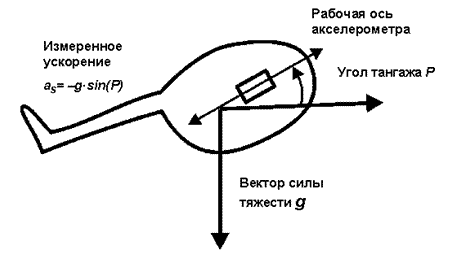
\includegraphics[width=0.6\linewidth]{pics/tangazh.png}}
\caption{Измерения величин крена и тангажа посредством акселерометров.}
\label{pic:tangazh}
\end{figure}

Полагая ускорение носителя равным нулю, мы можем вычислить угол тангажа как:
$$P = \arcsin (-a_s/g)$$

Аналогично вычисляется угол крена. Таким образом, два из трех углов, определяющих угловую ориентацию, могут быть определены только за счет использования акселерометров. Это совершенно очевидный результат, принимая во внимание то обстоятельство, что углы крена и тангажа по изначально определены по отношению к вертикали, которая в нашем случае соответствует вектору тяжести. Однако, здесь следует признать, что описанный метод не может быть использован на практике сам по себе, так как в описанной схеме существенно состояние покоя, в котором должна находиться система. Если это условие не соблюдается, то совершенно очевидно, что отсутствует принципиальная возможность выделить вектор ускорения свободного падения из суммы всех ускорений, которую испытывает система.

\textit{\textbf{Вычисление изменений ориентации с использованием гироскопов}}

Как отмечено выше, в конструкции навигационного комплекса используются оптические гироскопы, обладающие чувствительностью к изменениям ориентации т.е. к величине угловой скорости. Интегрирование (численное суммирование) значений, измеренных гироскопами, обеспечивает определение кратковременных угловых перемещений в физическом пространстве.

Для корректного расчета угла поворота должны быть учтены
внутренние ошибки гироскопа – дрейф, ошибка масштабного коэффициента, случайный шум.

При этом внутренние ошибки  гироскопа полностью смешаны с истинными значениями и не могут быть отделены от них на базисном информационном уровне. В процессе дальнейшей обработки эта смесь подвергается интегрированию, в результате чего возникает ошибочное угловое смещение, которое, таким образом, приобретает долговременный характер (рис. ~\ref{pic:acell}). Точная оценка величины ошибочного углового смещения и его устранение осуществляется при генерации навигационного решения на последующем навигационном уровне.

\begin{figure}[!htb]
\center{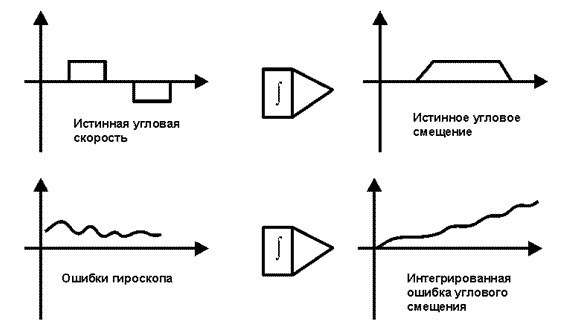
\includegraphics[width=0.6\linewidth]{pics/acelerometr.png}}
\caption{Схема определения углового смещения.}
\label{pic:acell}
\end{figure}

\textit{\textbf{Определение координат пространственного положения с помощью акселерометров.}}

Наличие акселерометров позволяет определять величины линейных ускорений, которые испытывает система. Положим, что ориентация системы в физическом пространстве определена точно с помощью методов, описанных выше. Тогда имеется возможность выделить вектор силы гравитации среди всей суммы векторов сил, приложенных к системе и, следовательно, оценить величину ускорения. Численное интегрирование ускорения позволяет перейти к скорости, а повторное интегрирование к перемещению. Таким образом, с учетом представленных выше замечаний и правилах перехода из физического пространства в географическое, появляется принципиальная возможность оценить геодезические координаты системы в любой момент времени.

\paragraph{Корректировка выходных данных}

\paragraph{Анализ функций, подлежащих автоматизации}

\subsubsection{Выбор критериев качества}
Выделим основные критерии, по которым следует оценивать разрабатываемую подсистему.
\begin{itemize}
\item \textbf{Необходимость в специальном оборудовании} - исходя из задачи, предполагается использование проектируемого модуля в низкобюджетных системах. В связи с этим необходимо обеспечить корректную работу подсистемы с неспециальным оборудованием таким, как бытовые камеры. 
\item \textbf{Стоимость необходимого оборудования} – исходя из предыдущего пункта, следует обеспечивать поддержку наиболее дешевого оборудования. 
\item \textbf{Сложность интеграции} – в современном мире наличия многих конкурентов и налогов одним из ключевых факторов при выборе между ними является простота использования продукта. В связи с этим необходимо снизить время, необходимое на интеграцию с разрабатываемой подсистемой, путем предоставления удобного в использовании API.
\item \textbf{Точность} - данный критерия является важным для задач определения положения в пространстве априори, так как при низкой точности использование систем данного рода становится бесмысленным. Тем не менее в рамках многих задач обеспечение чрезмерно высокой точности является избыточным.
\item \textbf{Возможность свободного использования} – нередко разработчики программных или аппаратных продуктов накладыают ограничение в виде разного рода лицензий распространения, которые ограничивают пользователей в распространении и использовании своих продуктов. В связи с этим важным явлется свободность использования продукта в любых целях, не  противоречящих законодательству стран, где проихсходит его использование.
\end{itemize}

\subsubsection{Анализ аналогов и прототипов}


\paragraph{Сравнительный анализ}

Для сравнения представленных вариантов воспользуемся методом взвешенной суммы. Данный метод позволяет объединить ряд критериев сравнения в один интегральный показатель, по которому затем выбирается наилучший вариант, соответствующий максимальному значению этого интегрального показателя. Метод взвешенной суммы можно представить следующим образом: 
$$ Y = \max_{j \ni m} \displaystyle\sum_{i=1}^{n} \alpha_i \cdot K_{ij},$$
где $\sum_{i=1}^{n} \alpha_i = 1$

По этому критерию проводится сравнение $j (j = 1, 2, …, m)$ вариантов по $i (i = 1, 2, …, n)$ показателям, где:

$n$ – количество показателей сравнения;

$m$ – количество вариантов сравнения.

$K_{ij}$ – нормированный коэффициент соответствия $i$-ого параметра $j$-ого варианта эталонному значению, т.е. для $j$-ого варианта:
$$ K_{ij} = \frac{\max_{j} X_{ij}} {X_{ij}}, $$
$$ 0 < K_{ij} < 1 $$
Соответствие систем-аналогов выбранным критериям качества представлено в Таблице

\subsubsection{Перечень задач, подлежащих решению в процессе разработки}

Исходя из приведенного выше первичного анализа предметной области можно сформировать список задач, подлежащих решению.

Необходимо решить следующие задачи:

\begin{enumerate}
\item разработка структуры и архитектуры подсистемы системы; 
\item разработка требований к формату и структуре передаваемых данных;
\item разработка алгоритмов обработки информации;
\item выбор и обоснование КТС, необходимого для реализации системы;
\item разработка графа диалога и набора экранных форм;
\item оценка предполагаемого качества функционирования системы;
\item организационно-экономическое обоснование разработки;
\item рекомендации по охране труда.
\end{enumerate}



